\documentclass[12pt,a4paper,english
% ,twoside,openright
]{tunithesis}

% Note that you must choose either Finnish or English here and there in this
% file.
% Other options for document class
  % ,twoside,openright   % If printing on both sides (>80 pages)
  % ,twocolumn           % Can be used in lab reports, not in theses

% Ensure the correct Pdf size (not needed in all environments)
\special{papersize=210mm,297mm}


% LaTeX file for BSC/MSc theses and lab reports.
% Requires the class file (=template) tunithesis.cls and figure files,
% either tut-logo, exampleFig (as pdf or eps) and example_code.c
% Author: Lucas Machado (2018)
% Based on TTU template by Sami Paavilainen (2006), modified by Heikki Huttunen (2014)


% More information about Latex basics:
% [Tobias Oetiker, Hubert Partl, Irene Hyna, Elisabeth Schlegl, The
% Not So Short Introduction to LATEX2e, Version 5.03, April 2014, 171
% pages.  Availbale: http://tobi.oetiker.ch/lshort/lshort.pdf]


%
% Define your basic information
%
\author{Chen Zhu}
\title{A Machine Learning Approach of Logistic Organ Dysfunction Score Estimation with Data Acquired from Bedside in ICU} % primary title (for front page)
\thesistype{Master's thesis} % or Bachelor of Science, Laboratory Report... 

% Put your thesis' main language last
% http://mirrors.ctan.org/macros/latex/required/babel/base/babel.pdf
\usepackage{lastpage}
\usepackage[english]{babel}
\usepackage[
backend=biber,
style=authoryear,
citestyle=authoryear,
autocite=inline
]{biblatex}
\usepackage{csquotes}
\usepackage{lscape} 
\usepackage{threeparttable}

\addbibresource{thesis_refs.bib} %Imports bibliography file

%
% You can include special packages or define new commands here at the
% beginning. Options are given in brackets and package name is in
% braces:  \usepackage{opt]{pkg_name}

% Option1) for bibliography does not need additional packages.

% Option2b) for bibliography: old way for using Name-year citations
% http://www.ctan.org/tex-archive/macros/latex/contrib/harvard/ 
%\usepackage{harvard}  


% Option3) for bibliography: newer way, esp. for Name-year citations
% http://www.ctan.org/pkg/biblatex
%\usepackage[style=authoryear,maxcitenames=2,backend=bibtex,
%  firstinits=true]{biblatex}
%% Note that option style=numeric works as well
%\addbibresource{thesis_refs.bib}

\definecolor{tunipurple}{RGB}{78, 0, 142}

% You can also add your own commands
\newcommand\todo[1]{{\color{red}!!!TODO: #1}} % Remark text in braces appears in red
\newcommand{\angs}{\textsl{\AA}}              % , e.g. slanted symbol for Ångstöm
\renewcommand{\thetable}{\arabic{table}}
% Preparatory content ends here



\pagenumbering{roman} % was: {Roman}
\pagestyle{headings}
\begin{document}



% Special trick so that internal macros (denoted with @ in their name)
% can be used outside the cls file (e.g. \@author)
\makeatletter



%
% Create the title page.
% First the logo. Check its language.
\thispagestyle{empty}
\vspace*{-.5cm}\noindent

\begin{figure}
    \vspace{-1.3cm}
    \advance\leftskip-2.5cm
    \noindent
\includegraphics{img/tunilogo.png}
\end{figure}
 
\vspace{2.5cm}
\begin{flushright}
\noindent\textsf{\LARGE{\@author}}

\noindent\vspace{0.5cm}

\noindent\Huge{\textsf{\textbf{\textcolor{tunipurple}{\@title}}}}
\end{flushright}
\vspace{10.7cm} % adjust to 12.7 this if thesis title needs two lines

% Last some additional info to the bottom-right corner
\begin{flushright}  
    \begin{spacing}{1.0}
      \textsf{Faculty of Information Technology and Communication Sciences (ITC)\\
      \@thesistype\\
      April 2023}
    \end{spacing}
\end{flushright}

% Leave the backside of title page empty in twoside mode
\if@twoside
\clearpage
\fi

% Turn off page numbering for the first pages
\pagenumbering{gobble}


% Some fields in abstract are automated, namely those with \@ (author,
% title, thesis type).

\chapter*{Abstract}

\begin{spacing}{1.0}
\noindent \@author: \@title\\
\@thesistype\\
Tampere University\\
Master’s Degree Programme in Software Development\\
April 2019
\end{spacing}
\noindent\rule{12cm}{0.4pt}

\vspace{0.5cm}

% ---------------------------------------
% Abstract and keywords
% ---------------------------------------

\noindent Logistic Organ Dysfunction Scale (LODS), with weighted variables with the worst values in first 24h, is an organ dysfunction score system which reflects severity level within an organ system and among organ systems. It is considered as an outcome risk prediction scoring system as well, since an equation is included that converts LODS into probability of mortaility. In some research, it is confirmed to be usable for the first 7 days in ICU, and is widely used in other departments as well. LODS calculation needs some labrotary results, such as bilirubin, which cost time and money.

\noindent This thesis is to propose a machine learning model to predict LODS with data that can be accquired from bedside in first 12 hours of ICU stay, to save time and assist doctor in treatment.




~

\noindent\textbf{Keywords:} machine learning, organ dysfunction score.

~

\noindent The originality of this thesis has been checked using the Turnitin Originality Check service.


% Add the table of contents


\setcounter{tocdepth}{3}              % How many header level are included
\tableofcontents                      % Create TOC


% The actual text begins here and page numbering changes to 1,2...
% Leave the backside of title empty in twoside mode
\if@twoside
%\newpage
\cleardoublepage
\fi


\renewcommand{\chaptername}{} % This disables the prefix 'Chapter' or
                              % 'Luku' in page headers (in 'twoside'
                              % mode)


\chapter{Introduction}
\label{ch:intro} 

\pagenumbering{arabic}
\setcounter{page}{1} % Start numbering from zero because command
                     % 'chapter*' does page break
                     
% \label{...} allows cross-referencing, e.g. 'as explained in
% Chapter~\ref{ch:intro}' Note that you may have to run the command
% 'latex' or 'pdflatex' twice to get cross-references correctly.  You
% can add labels e.g. to chapters, sections, figures, tables, and
% equations.

% You can write everything into single tex file. Alternatively, you
% can write each chapter into separate file and then include them her
% \include{intro} % no postfix .tex to the command
% \include{related_works} % and so on...

Since the first intensive care unit (ICU) established in Denmark in 1953, the ICU has become an essential element in hospital-care based health care. An intensive care unit is defined as an organized system to treat critically ill patients with intensive and specialized medical and nursing care, an enhanced capacity for monitoring, and multiple methods of physiologic organ support to sustain life when patient has acute organ system insufficiency. An ICU's activities are not limited to the geographic area in a hospital, but extend to include emergency department , hospital ward and follow-up clinic. \parencite{Marshell2017} Patients with critical illness might be found throughout a hospital, however, many of them are treated in ICU. ICU mortality varies by different conditions, for instance, according to \textcite{Adhikari2010}, 8-18\% in unselected patients in North America, Europe, Australia, and New Zealand, 35–45\%48 in heterogeneous cohorts of patients with acute lung injury, and 50–60\%49 in patients with septic shock. Patients in ICU are in three main categories: those with acute organ dysfunction (including those who receives long-term intensive organ support because of their unclear ultimate outcome), those who had a major procedure and are monitored in the peri-intervention period, and those who are receiving end-of-life care. To give sufficient but not excessive treatment, ICU is divided into different levels. A level 1 provides oxygen, noninvasive monitoring, and more intensive nursing care than on a normal ward, where a level 2 ICU is capable to provide invasive monitoring and basic life support for a short period. A level 3 ICU serves as a regional resource for critically ill patients by providing a full spectrum of monitoring and life support technologies. It may play an active role in developing the specialty of intensive care through research and education. \parencite{Marshell2017} Patients, families and care providers concern recovery likelihood, however, prognostication can be difficult in ICU. Scoring systems are used to objectively quantify condition severity and risk stratify patients for prognostication in clinical. They are also used as standard tools in critical care research to demonstrate equivalence of patients group. \parencite{Tiffany21}

Scoring systems are tools used in critical care to clinically objectively quantify severity, risk stratify patients for clinical prognostication and in research as study inclusion criteria and to demonstrate equivalence of patient groups. It can broadly be divided into those that are specific for a disease or an organ, for example the Glasgow Coma Scale, and those that are for all ICU patients. The scores that are generic for all ICU patients are broadly divided into: 1) scores that assess severity on admission and predict outcome, for example, Acute Physiology and Chronic Health Evaluation (APACHE), 2) scores that assess the severity of organ dysfunction, for example, Sequential Organ Failure Assessment (SOFA), 3) scores that assess nursing workload using, for example, Nine Equivalents of Nursing Manpower Use Score (NEMS). \parencite{Tiffany21, Jonathan2008, Rapsang2014, Vincent2010} Logistic Organ Dysfunction Score \parencite{legall96}, as somewhere between mortality prediction score and organ dysfunction score, is developed to assess and characterize current degree of organ dysfunction. \parencite{Tiffany21, Vincent2010} It selects 12 variables to represent the function of six organ systems, which include laboratory results and non-invasive parameters. It ranges from 0 to 22 where 0 is no dysfunction and 22 is maximum dysfunction. It also included a logistic regression equation that can convert the score into a probability of mortality. Although it was not initially validated for repeated use in ICU, \textcite{Timsit2002} validated that LODS characterized the progression of organ dysfunction accurately in the first 7 days of ICU stay.

Machine learning is a branch of artificial intelligence, broadly defined as the capability of a machine to imitate the way that human learns. It is the foundation behind predictive text, language translation apps, and the way social media feeds are presented. \parencite{sara2021} Quoted to \textcite{samuel1959}, machine learning is that computers can be given the ability to learn without being explicitly programmed. What this means is that a computer program learns with observed data and a learning algorithm to perform a task, such as predicting result. Generally, data in machine learning is split to two groups, a training set and a test set. As the name suggests, the training set is used to train algorithm where features are included. The test set is used to algorithm performance and it is new to the algorithm. Once an algorithm passes the training and test phases with an acceptable performance, it will be implemented to real world. The adoption of machine learning can be found in science, commerce and technology, including the diagnosis of faults in complex systems and consumer services. \parencite{jorden2015} In healthcare, machine learning has evolved for years. It is capable to assist case triage, enhance image scanning and segmentation, and support decision making, and it has changed and will shift healthcare epidemiology, for example, predicting risk of Nosocomial Clostridium difficile Infection (CDI) and predicting clinical outcomes in Ebola Virus Disease (EVD) Infection using initial clinical symptoms. \parencite{Jenna2017, Habehh2021} In addition, machine learning is applied a lot in electronic health records (for example, analys heart failure survival \parencite{Panahiazar2015}), medical imaging (for example, detecting diabetic retinopathy from retinal photographs \parencite{Gulshan2016}), and genetic engineering (for example, predicting the immunogenic landscape of SARS-CoV-2 \parencite{Malone2020} ).

Medical score system needs accuracy to reflect patients’ condition, and ease of use to reduce clinician time in using and learning. Only if a score system is substantially better than another one, proved by a large number of research, it will be used in practice. So improving an existed score system is more feasible than replacing, and change should be small but useful. LODS esitmates with the worst value of the first 24 hours of ICU stay, both bedside and laboratory measurements, which cost money and time. This research would use only bedside data because they are easy to access, without long-time waiting or money cost. And for some dangerous patients, 24 hours is a long time to collect data. If 24h severity can be predicted early, doctors will be able to change the treatment. LODS is a hybrid scoring system which makes it a good tool in this prediction. As human physiology comprises a complex system, using mathematical models to analyse organ dysfunction may describe systemic host response to infection or injury. \parencite{seely2011} So in this research, machine learning is brought to bedside to predict patients' severity by predicting LODS. ICU has many monitoring devices and produces a large amount lab test results which is a great resource for machine learning model training and research.


chapter information

This document is structured as follows. Chapter~\ref{ch:style}
discusses briefly the basics of writing and presentation style
regarding the text, figures, tables and mathematical
notations. Chapters~\ref{sec:ref_styles} and \ref{ch:concl} summarize
the referencing basics and the whole document. There are two example
appendices as well (Appendix A and B).
% ~\ref{app:A} and \ref{app:B}). Labels do not with \chapter*

\chapter{Background}
\label{ch:background}

chapter target
\section{Severity Scoring systems}
In critical care, physiology-based scoring systems applied much more than diagnosed-based scoring systems, because sometimes no diagnoses are made on admission and patients in ICU can have more than one organ failure where diagnose-based scoring system is inapplicable. \parencite{Bouch2008} Severity scores are divided into those calculated with data obtained in the first day of ICU admission (for example, the mortality prediction model (MPM)), and those calculated with data collected sequentially throughout the duration of ICU stays (for example, the Sequential Organ Function Assessment (SOFA)). 

Both first day and sequential systems can be divided into subjective scores and objective scores. Subjective scores are established by taking variables and applying weights on them based on personal experience of a panel of experts. A range of normality is defined for each variable. The higher weights are assigned to more abnormal results, mostly from 0 to 4. The final score is the total number of points. For instance, Sequential Organ Failure Assesssment (SOFA). Objective scores are developed from a large database of clinical data which is compiled from many ICUs. A multipurpose probability model will be applied to determine ranges, assign weights, and select variables. Variables can be classified into four groups: age, comorbidities, physiological abnormalities, and acute diagnoses. Outcome of these systems are on vital status at hospital discharge predominantly and other measures (for example, life among long-term survivors and vital status 28 days after hospital discharge or quality). All systems result in a logistic regression model to estimate or assist in estimating the risk of death. \parencite{LeGall2005, Bouch2008} 

The principle use of severity scoring systems is to predict and evaluate individual patient's situation. Outcome prediction scores and organ dysfunction are two main categories of severity scoring system, which are respectively used to objectively predict risk of death and assess organ dysfunction. Outcome prediction score was originally developed to provide an indication of the risk of death of groups of ICU patients. However, with the development of medical data and practice, include patient demographics, disease prevalence, and intensive care practice, and statistical and computational techniques, the updated versions of those scores can be applied to individual patient. For instance, the four versions of Acute Physiology and Chronic Health Evaluation (APACHE)  are widely used in ICUs worldwide. Organ dysfunction scores are primarily designed to describe the degree of organ dysfunction. The severity of organ dysfunction varies from one individual patient to another and over time for one individual. Organ dysfunction should take both time and severity into account. There is not a score that covers all organ systems. Moreover, for all organ systems that one score covers, accuracy might varies. \parencite{LeGall2005, Bouch2008, Vincent2010} Severity score systems give assistance in clinical decisions by its objectivity, although they are not always accurate. It's prudent to use severity systems in decision-making, instead of only subjective opinion. But according to \textcite{LeGall2005, Vincent2010-at}, severity scores should not be used to dictate individual patient decisions. In addition, severity scores are also used in clinical trial (for example, evaluating how organ dysfunction affects sepsis morbidity), and evaluation of ICU performance (for example, comparing the probabilities of hospital mortality and actual outcome in ICUs in several countries). \parencite{LeGall2005, Vincent2010}

This research focus on Logistic Organ Dysfunction Score, an organ dysfunction score which is originally designed for first-day use in ICU.

\subsection{Logistic Organ Dysfunction Score}
Logistic Organ Dysfunction Score, acronym as LODS, is initially proposed by \textcite{legall96}. The initial goal was to propose an objective system that can reflect  patient severity adequately, and as simple as possible to apply.  In many scoring systems, each organ system is graded from 1 to 4 or from 1 to 6, which are different from the ranges found using statistical methods. Moreover, all organ systems are weighing in the same way does not take the differential prognostic significance of the involved organs into account. 

LODS was proposed with the large database of the European-North American study (ENAS), where 14,745 consecutive admissions in 137 medical, surgical, or mixed ICUs in 12 countries. Only patients aged 18 years or older were eligible; burn patients, coronary care patients, and cardiac surgery patients were excluded. Twelve variables were selected by multiple logistic regression to represent the function of six organ systems (neurologic, cardiovascular, renal, pulmonary, hematologic, hepatic). The worst value for each variable within 24 hours of ICU admission are ranked to a scale that considers no dysfunction with 0 to maximum dysfunction with 5. LODS is a weighted system: the maximum score allowed for the respiratory and coagulation is 3, and the maximum score for liver is 1. Therefore, LODS value ranges from 0 to 22, as Table \ref{table:lods}. For sedated patients, the GCS was ascertained either by reviewing the patients' medical record before sedation, or from interviewing the physician who ordered sedation. A variable was assumed to be normal if it was not measured. All variables were continuously scaled except platelet count and prothrombin time. The worst value of first 24h refers to the worst recorded values that received the highest number of LOD points. For example, if a patient at different has tachycardia of 150 beats per minute (1 LOD point) and bradycardia of 25 beats per minute (5 LOD points), 5 is recorded for cardiology. LODS is considered as a hybrid organ dysfunction and outcome risk prediction scoring system as it combines a global score summarizing the total degree of organ dysfunction of the organ systems, and a logistic regression equation that can convert the score to a probability of mortality (e indicated to a mathematical constant 2.7182818). Within organ systems, higher mortality is associated with greater severity scores, that a LODS of 22 is associated with a mortality of 99.7\%. \parencite{Tiffany21, Vincent2010, sekulic2015}

\begin{equation*}
Predicted Death Rate = (e^{-3.4043 + 0.4173*(LODS)} ) / ( 1 +  e^{-3.4043 + 0.4173*(LODS)} )
\end{equation*}

LODS was originally developed for the first 24 hours of ICU stay, but it is also validated as an accurate organ dysfunction score in the first 7 days of ICU stay by \textcite{Timsit2002} in a study of 1,685 patients in French ICUs. \textcite{Metnitz2001} confirmed that LODS is well correlated with the numbers and levels of dysfunctions, and well in discriminating survivors and non-survivors in a study with 2893 consecutive admissions in ICU in Austria, from which LODS was considered to provide combined measure of morbidity and mortality for patients critically ill with multiple organ dysfunction/failure. \textcite{Blanco2008}  proved that total LODS score was associated with early death of patients with severe sepsis in ICU.


\begin{landscape}
    \begin{table}[]
    \begin{threeparttable}
        \caption{Logistic Organ Dysfunction Score.}
        \label{table:lods}
        \begin{tabular}{lllllllll}
            \hline
            \textbf{Organ system} & \textbf{Parameter} & \textbf{5} & \textbf{3} & \textbf{1} & \textbf{0} & \textbf{1} & \textbf{3} & \textbf{5} \\
            \hline
            Neurologic & GCS\tnote{1} & 3-5 & 6-8 & 9-13 & 14-15 & - & - & - \\
            Cardiologic & HR\tnote{2} (beats/min) & \textless 30 & - & - & 30-139 & 140 & - & - \\
             &  &  & or &  &  & and & or &  \\
             & SBP\tnote{3} (mmHg) & \textless 40 & 40-69 & 70-89 & 90-239 & 240-269 & $\geq$270 & - \\
            Renal & Urea nitrogen (mmol/l) & - & - & - & \textless{}6 & 6-9.9 & 10-19.9 & $\geq$20 $\geq$ 1.20 \\
             & (g/l) &  &  &  & \textless{}0.36 & 0.36-0.59 & 0.60-1.19 &  \\
             &  &  &  & and & or & or &  &  \\
             & Creatinine ($\mu$mol/l) & - & - & - & \textless{}106 & 106-140 & $\geq$141 & - \\
             & (mg/dl) &  &  &  & \textless{}1.20 & 1.20-1.59 & $\geq$1.60 &  \\
             &  &  &  & and &  & or &  &  \\
             & Urine output (l) & \textless{}0.5 & 0.5-0.74 & - & 0.75-9.99 & - & \textgreater{}=10 &  \\
            Pulmonary & PaO2 mmHg/FiO2 (on MV or CPAP) &  & \textless{}150 & $\geq$150 & no MV no CPAP & - & - & - \\
             & PaO2 kPa/FiO2 & - & \textless{}19.9 & $\geq$19.9 & no IPAP & - & - & - \\
            Hepatic & Bilirubin ($\mu$mol/l) & - & - & - & \textless{}34.2 & $\geq$34.2 & - & - \\
             & (mg/dl) &  &  &  & \textless{}2.0 & $\geq$2.0 &  &  \\
             &  &  &  &  & and & or &  &  \\
             & PT\tnote{4}time (secs) & - & - & - & $\leq$3 & \textgreater{}3 & - & - \\
             & above standard (\%) &  &  & \textless{}25 & 25 &  &  &  \\
            Hematologic & Leukocytes (× 10 9/l) & - & \textless{}1.0 & 1.0-2.4 & 2.5-49.9 & $\geq$50.0 & - & - \\
             &  &  &  & or & and &  &  &  \\
             & Platelets (109/l) & - & - & - & \textless{}50 & \textgreater{}=50 &  &  \\
             \hline
        \end{tabular}
        \begin{tablenotes}
            \item[1] GCS: Glasgow coma scale; 
            \item[2] HR: heart rate; 
            \item[3] SBP: systolic blood pressure;        
            \item[4] PT: prothrombin
        \end{tablenotes}
        \end{threeparttable}
    \end{table}
\end{landscape}


\section{Machine Learning}
Machine learning is a branch of computational algorithms that are designed to learn from experience to emulate human intelligence. \parencite{elnaqa2015} It uses input data to achieve a desired task without being literally programmed to produce a specific outcome. The algorithms adaptively alter their structure to improve performance as the data increases. Machine learning is the core of artificial intelligence and data science, and lies at the intersection of statistics and computer science. \parencite{jorden2015} 

Over the past two decades, machine learning has developed dramatically from laboratory to commercial use. It broadly affects across computer science and industries concerned with data-intensive issues, such as consumer services and the diagnosis of faults in complex systems. Similarly, a range of empirical sciences are also affected, from biology to cosmology to social science, as machine learning methods have been developed to analyze experimental data in novel ways. \parencite{jorden2015}

A large amount of algorithms has been developed to cover different data and problem types in machine learning problems.


machine learning situation,
electric devices with much data produced in icu stays.



\chapter{Prior Work}
\label{ch:priorwork}
Mathematics and machine learning have been brought to ICU severity prediction and estimation in many research, however, most of them focus on combine laboratory and vital sign measurements together to predict mortality. There are some studies that use bedside data to estimate or predict patients' situation.

\textcite{asuroglu2021} proposed a deep learning approach to monitor sepsis onset by predicting Sequential Organ Function Assessment (SOFA) score with seven vital signs of 12 hours that can be acquired from bedside in Intensive Care Unit (ICU), include heart rate, systolic and diastolic blood pressure, respiratory rate, oxygen saturation, Glasgow Coma Scale eye opening (GCS) and temperature. The experiments used a subset of Medical Information Mart in Intensive Care (MIMIC) III dataset. It consists of 53423 ICU records of patients who are older than 15 from 2001 to 2012 at Beth Israel Deaconess Medical Center (BIDMC) in Boston, Massachusetts. In Asuroglu's experiments, 5154 samples are extracted as input which have seven different vital signs and meet three additional inclusion criteria, (1) a sepsis onset time should be predictable, (2) there is at least one available measurement for each of vital signs 12 hour prior to predict onset time, (3) an artificial onset time was determined which include patients without sepsis. He used these samples to train a model to predict SOFA score, which is used to evaluate sepsis now. Probabilistic Principal Component Analysis (PPCA) is used to impute missing value in the dataset. It combines Principle Component Analysis (PCA) with a probabilistic approach and Expectation-Minimization approach method. To achieve the goal, Asuroglu combined Convolutional Neural Networks (CNN) features with Random Forest (RF) algorithm, where CNN is used as a feature extraction tool and Random Forest is used to make a final decision. Correlation Coefficient (CC), Mean Absolute Error (MAE) and Root Mean Square Error (RMSE) were used to assess the prediction performance. As a result, the model has the best performance when compared with other models, like Bi-LSTM and Linear Regression, with 1.23 as RMSE, 0.659 as MAE and 0.863 as CC.

\textcite{johnson2013} used 10 bedside variables to propose a score system called Oxford Acute Severity of Illness Score (OASIS) to estimate patients' situation in the first day of ICU stay, include pre-ICU length of stay, age, Glasgow Coma Scale (GCS), heart rate, mean arterial pressure (MAP), respiratory rate, temperature, urine output, ventilated or not and elective surgery or not. It uses the worst value of the variables in the first 24 hours in ICU stay, which conduct a scale from 0 to 73. OASIS also includes an equation to convert score to mortality. The objective of the study was to use a machine learning technique which is called particle swarm optimization to reduce the number of parameters collected in Acute Physiology, Age, and Chronic Health Evaluation (APACHE) IV system with no predictive accuracy lost. The data of this study, 81,807 admissions, was a subset of data obtained from 86 ICUs at 49 hospitals that had installed an APACHE IV system from January 1, 2007 to September 15, 2011. Patients with burn, stay in ICU less than 4 hours and younger than 16 are excluded from the dataset. Posttransplant patients, other than hepatic or renal transplantation, are excluded from the research. there are 8613 admissions were removed because of the missing variables, resulting in a final cohort of 72,474 admissions, which was divided into development dataset (39,070 admissions), internal validation dataset (9,786 admissions) and external validation dataset (23,618 admissions). Genetic Algorithm (GA) was used to select variables, and particle swarm optimization was used to determine the weight assigned to each variable. A research in China validated that OASIS have better accuracy than Sequential Organ Function Assessment (SOFA) and Logistic Organ Dysfnction Score (LODS) in mortality prediction of patients with sepsis in ICU. \parencite{hu2020} \textcite{el-manzalawy2021} used 10 variables of OASIS and machine learning model to propose a new OASIS+ score system.


AALTO thesis
chinese with non-invasive parameters

\chapter{Methods}
\label{ch:methods}

\section{Dataset}
The Medical Information Mart for Intensive Care (MIMIC)-IV database version 2.2 is used in this research. \parencite{johnson2023} The MIMIC IV dataset is the updated version of the MIMIC III created in 2020. It comprises deidentified health-related data from patients who were admitted to the critical care units of the Beth Israel Deaconess Medical Center (BIDMC) in 2008-2019 in Boston Massachusetts. The dataset consists of 73,181 ICU stay records, vital sign and laboratory measurements of these records are all included. MIMIC IV is deidentified and patient identifiers were removed according to the Health Insurance Portability and Accountability Act (HIPAA) Safe Harbor provision.

A waiver of informed consent and approved the data sharing initiative by the Institutional Review Board at the Beth Israel Deaconess Medical Center, who reviewed the collection of patient information and creation of the research resource. \parencite{johnson2023}


\section{Missing Data Imputation}
\subsection{Linear}
\subsection{PPCA}
\subsection{Multi Imputation}
\section{Models}
\subsection{XGBoost}
\subsection{Random Forest}
\section{Correlation}

\chapter{Experiments}
\label{ch:experiment}

\chapter{Results}
\chapter{Conclusion}
\chapter{Discussion}



\chapter{Writing style}
\label{ch:style}

Effective written communication requires both sound content and clear
style. Keep the layout of your thesis neat and pay attention to your
writing style.

\section{Using LaTeX}

This document serves as an example, rather than tutorial, since there
are plenty of those available, see for example 
\cite{Dummy:1,oetiker14, latex13}. The source files are compiled
with the command \texttt{pdflatex d\_tyo.tex} (or \texttt{latex
  d\_tyo.tex}). Depending on your bibliography style, you might also
need to run \texttt{bibtex d\_tyo}.

Unfortunately, compilation may fail, if your LaTeX environment does
not have all the needed packages installed. If you cannot install
them, you can momentarily disable them by putting them inside comments
in the file tutthesis.cls:
\begin{center}
\texttt{\% \textbackslash usepackage\{hyperref\}}
\end{center}
Of course, depending on the package, some of the features are also
disabled and you must remove those parts from your tex file.
Spellchecking can done, for example, by running 
\texttt{aspell -t -c d\_tyo.tex}.

Moreover, certain characters need escape symbols, e.g. per cent should
be written as \textbackslash\% (otherwise it starts a comment),
underscore as \textbackslash\_, tilde as \textbackslash\~{}\{\}, hash
as \textbackslash\#, dollar sign as \textbackslash\$, and opening
brace as \textbackslash\{ and so on. Note that double backslash
\textbackslash\textbackslash makes a line break.

\section{Text}
A thesis is written with a single-column layout on one- or two-sided
A4 sheets (210 mm x 297 mm). The font type of the body text is usually
Times New Roman and the font size is 12 pt. The spacing is 1.2 and the
text is fully justified and hyphenated. You do not have to indent the
paragraphs.

Arial 18 pt font is used for the headings in this guide, and there is
a 42 pt space above and below. The font size of subheadings is
14. There is an18 pt space above subheadings and 12 pt space below
them.
\\
Brief basics of writing style are:
\begin{itemize}
\item Always think of your reader when you are writing and proceed
  logically from general to specific.
\item Highlight your key points, for example, by discussing them in
  separate chapters or presenting them in a table or figure. Use
  \textit{italics} or \textbf{boldface} for emphasis, but don't overdo
  it.  Moreover, this template uses \texttt{teletype} font for LaTeX
  specific names, such as commands and files.
\item Avoid long sentences and complicated statements. A full stop is
  the best way to end a sentence.
\item Use active verbs to make a dynamic impression but avoid the
  first person pro-noun ``I'', except in your preface.
\item Avoid jargon and wordiness. Use established terminology and
  neutral language.
\item The minimum length of chapters and subchapters is two
  paragraphs, and you need to consider the balance of
  chapters. Paragraphs must always consist of more than one sentence.
\item Do not use more than three levels of headings, such as 4.4.2.
\item Do not use too many abbreviations. Use capital and small letter
  consistently
\end{itemize}

Sometimes ending a section with list is considered as bad
style. Therefore, it is better to have some text after it.


\section{Figures}
You must refer to all the figures in the body text. The reference
should preferably appear on the same page as the actual figure or
before it. Figures and tables must be numbered consistently thesis
and primarily placed at the top of the page, but you are free to
decide where they fit best. Never start a chapter with a figure, table
or list.

Figures and the caption are either consistently centered (or aligned
to the left). The caption is placed under the figure and always on the
same page as the figure. All figures must be explained in the body
text, so that readers know what they are supposed to notice. Figures
generated by analysis software usually need further editing, see
Figure~\ref{fig:ex_fig} for example. The figures should be in the same
language as other text (even if Figure~\ref{fig:ex_fig} violates this
recommendation). The recommended font size is the same as that of the
body text but no smaller than 10 pt. The figures must be readable,
even if your thesis is printed in greyscale.
% Note: put tilde between text and ref command, like in
% 'Figure~\ref{fig:ex_fig}' above. Tilde (~) puts a white space but
% prevents line break. Same thing applies to Table~\ref{tab:summary}
% as well.

% Here's an example how to add a figure. Default placement of figures
% is at top of page, i.e. placement specifier is '[t]' could be
% omitted.  The dimensions can be relative to text width (or height)
% or absolute (4 cm).

% You can leave out the figure postfix (.pdf, .eps, .png). Utilized
% tool (pdflatex, latex...) decides what file type to look for.
% http://en.wikibooks.org/wiki/LaTeX/Importing_Graphics#Compiling_with_latex

% Note that figure is placed _after_ this point and also after the
% previous figures. You can cut-paste the figure insertion point
% earlier to get it in better place, i.e. the figure can be before
% reference to it in the Tex file, but otherway round in final pdf.
% More information: [Oetker, pp. 49-52]. 
\begin{figure}[t]
  \begin{center}
    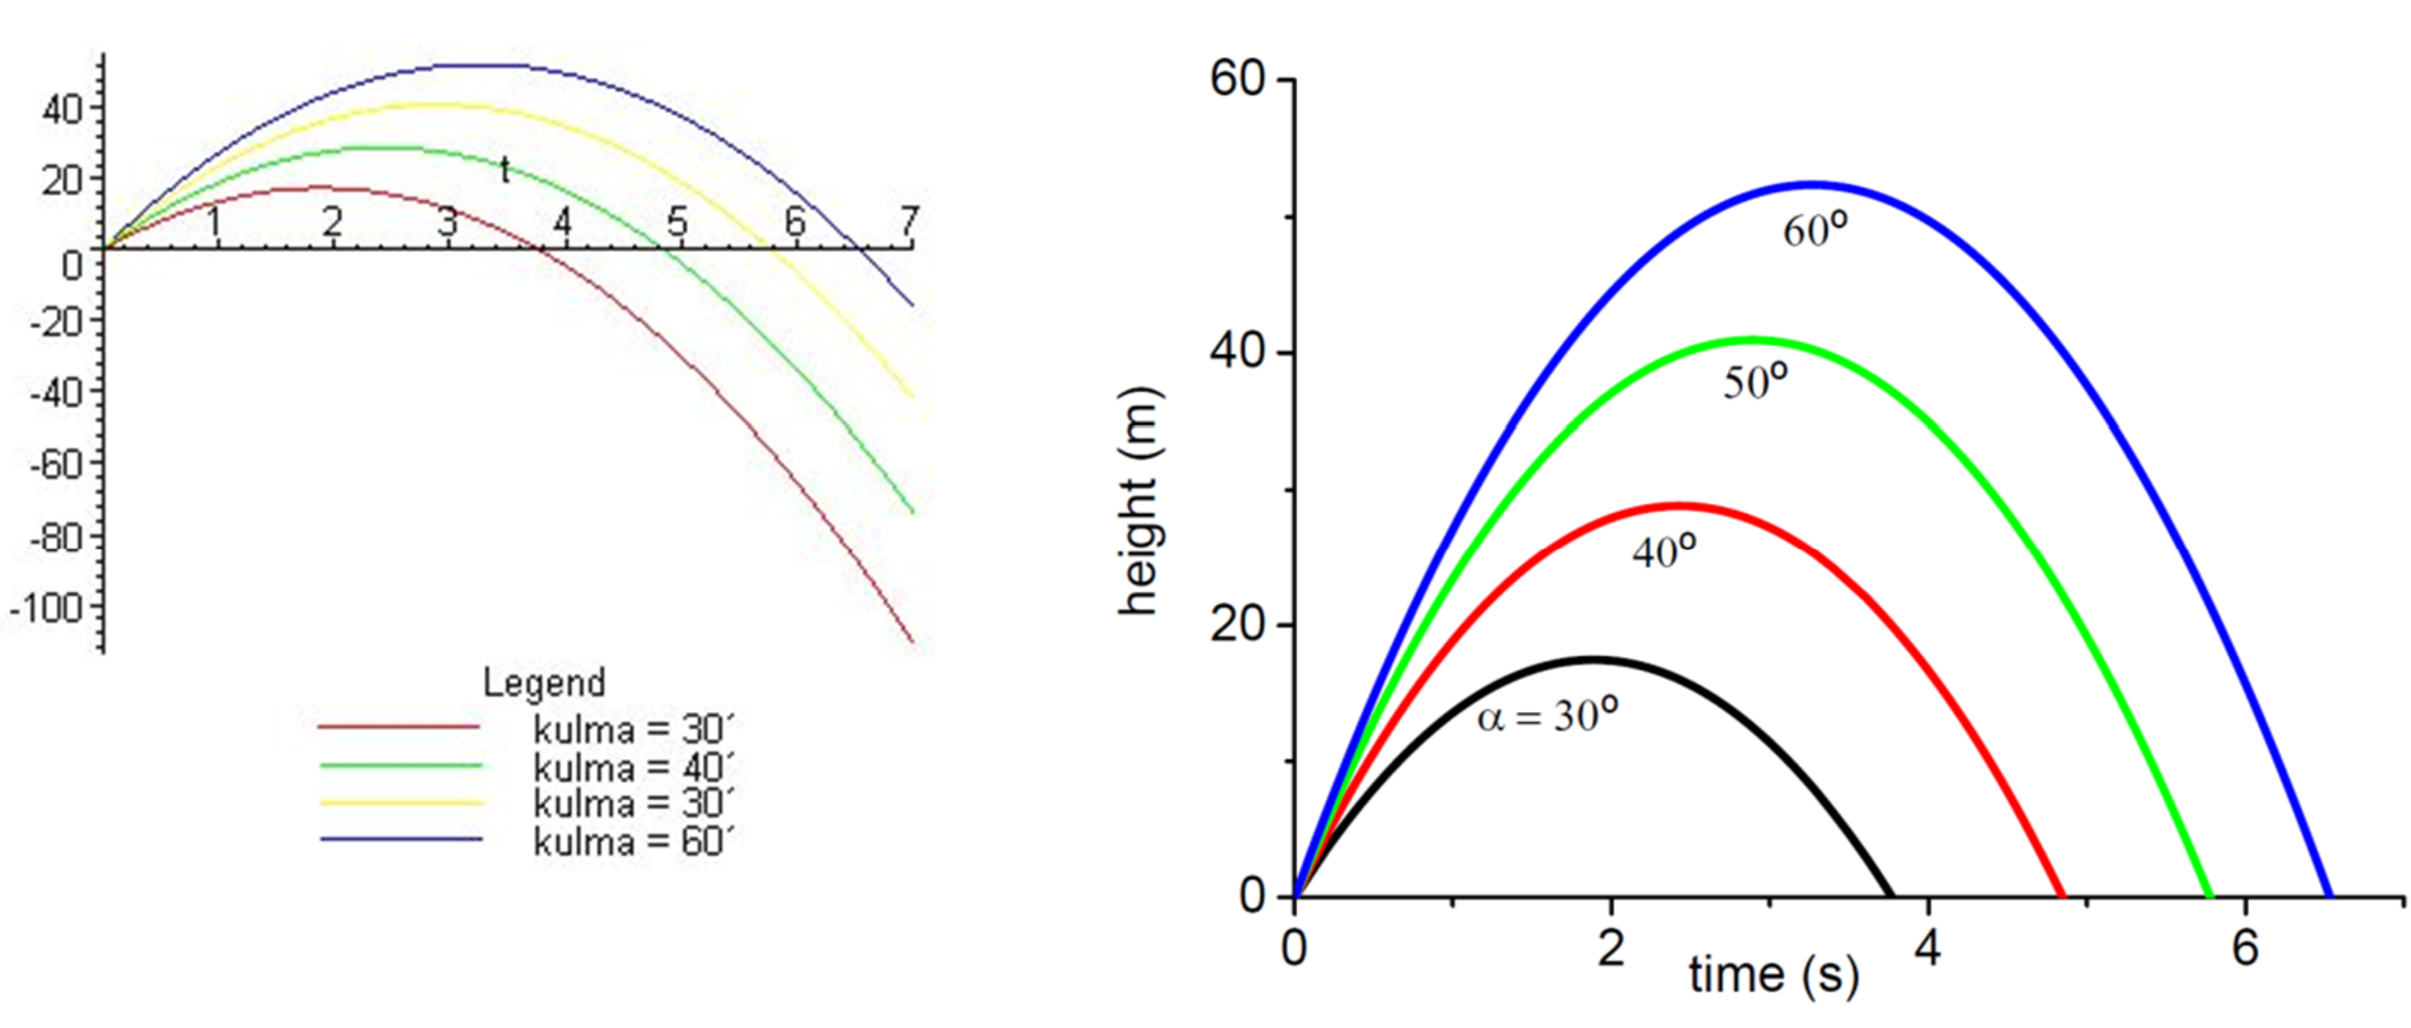
\includegraphics[width=1.0\textwidth]{exampleFig}
  \end{center}
  \caption[Diagrams should be edited before publication.]{Diagrams
    should be edited before publication. The diagram on the right is
    an edited version of the one on the left.}
  % Optional shorter caption in brackets is used in Table of Figures
  % (tof).
  \label{fig:ex_fig}
\end{figure}

% In conference and journals articles with two columns, the
% command \begin{figure*} is useful. The asterisk makes the figure
% width equal to the whole page. The same applies to \begin{table*} as
% well.



The basic command \texttt{latex} accepts only encapsulated postscript
(eps) format. Therefore it is usually easiest to compile with
\texttt{pdflatex} which can handle \verb+*.png+, \verb+*.jpg+ and
\verb+*.pdf+ formats. Eps and pdf are recommended since their support
vector graphics (zooming). For example Figure~\ref{fig:ex_fig} is in
pdf format. 
%Some programs, such as PowerPoint, store pdf figures A4
%sized. Fortunately, pdf editors, such as PDF-X-Change, have a feature
%'remove white spaces' or 'crop'.


LaTeX has a package \texttt{subfigure} to layout multiple figures
together, for example Figure~\ref{subfig:draft} to
\ref{subfig:small_fig}. There might be newer packages as well, but this is
already a quantum leap ahead of some other, unnamed word processors.
% See http://www.ctan.org/pkg/subfigure
\begin{figure*}
  \begin{center}
    \subfigure[Option \texttt{draft} helps to makes a placeholder box for figure. The file must exist.]{
      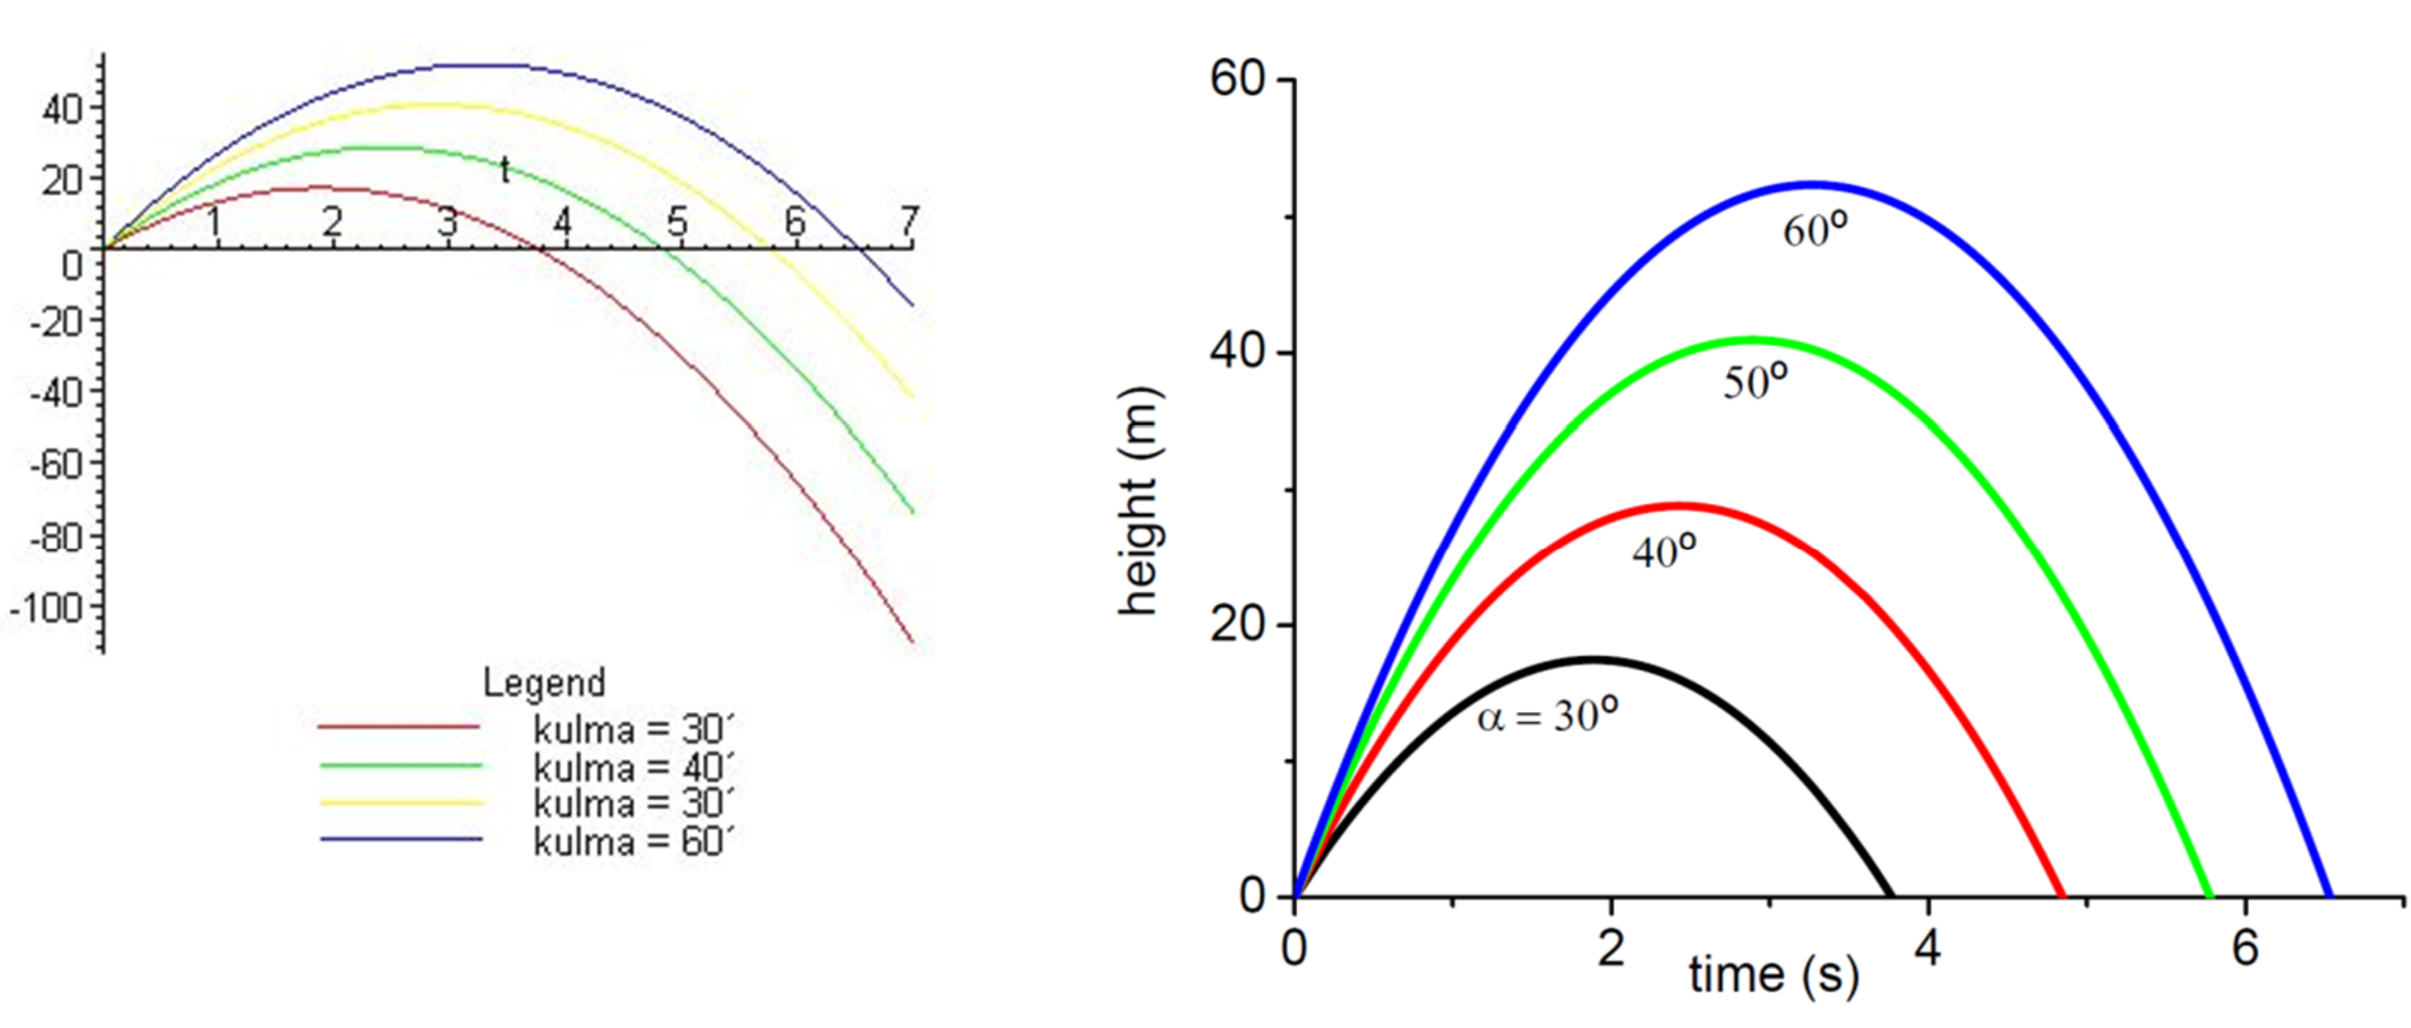
\includegraphics[draft, width=0.35\textwidth]{exampleFig}
      \label{subfig:draft}}
    \qquad                        % i) Ugly hack to get more horizontal space between figures
    %\hspace{0.05\textwidth}      % ii) Another ugly way to hack space
    % ~~                          % iii) Yet another... 
    \subfigure[Another way ot make a placeholder box with the command
      \texttt{rule}.]{
      \textcolor{blue}{\rule{0.3\textwidth}{3cm}}
      \label{subfig:rule}}
    \subfigure[Actual figure included but scaled down.]{
      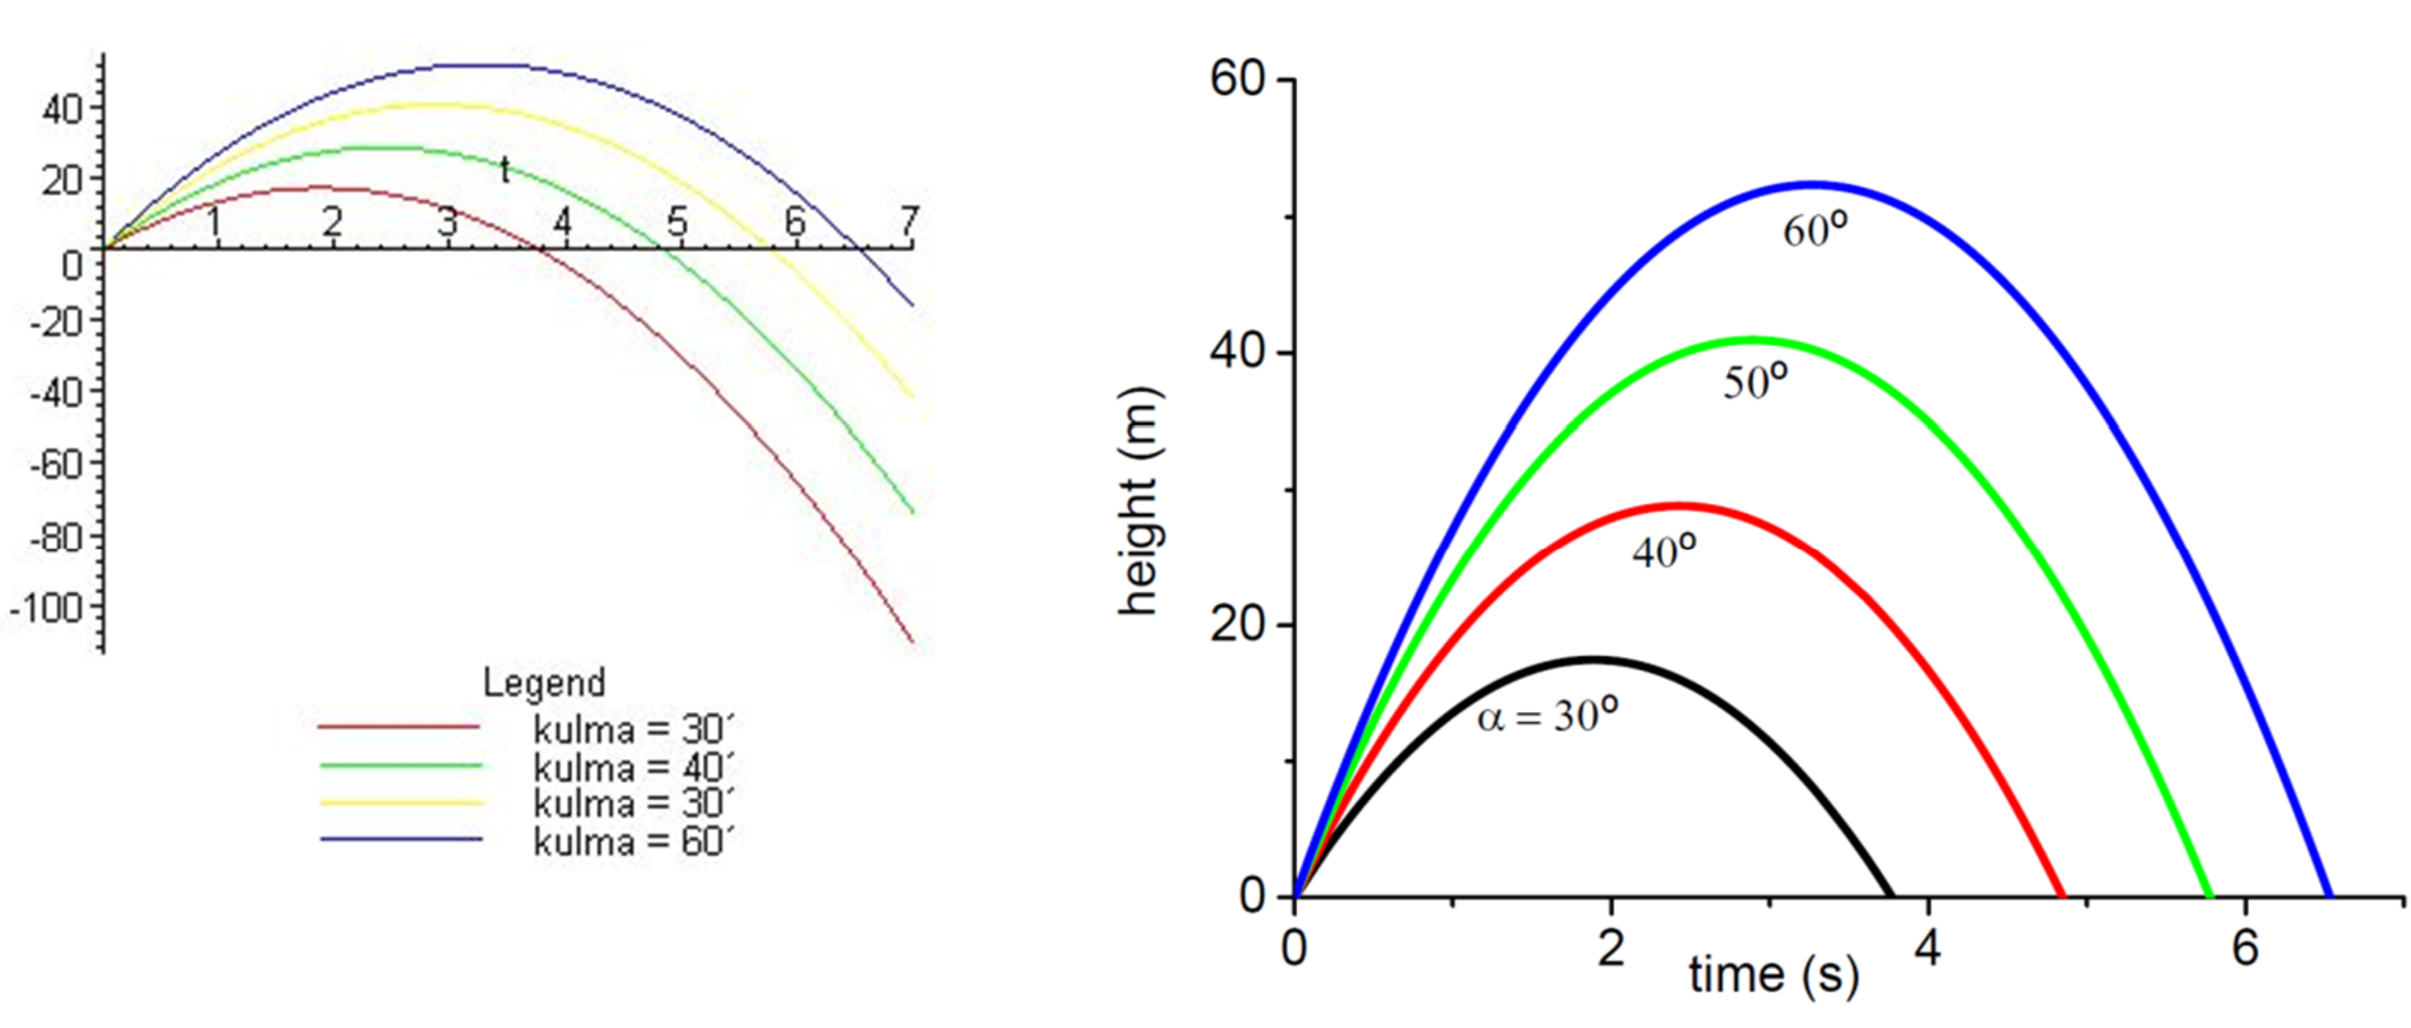
\includegraphics[width=0.35\textwidth]{exampleFig}
      \label{subfig:small_fig}}
    \caption[Example of subfigures]{Example of subfigures. Pay attention to how nicely they
      are laid out and their neat subcaptions.}
    % Optional shorter caption in brackets is used in Table of Figures
    % (tof).

    \label{fig:subfigs}
  \end{center}
\end{figure*}


\section{Tables}

Tables have numbered captions, see Table\ref{tab:thin_film} for
example. The caption is placed on the same page but above the table,
unlike the captions that accompany figures. You must refer to all the
tables in the body text. In addition, you must discuss the content of
any tables in the body text to ensure that readers understand their
relevance.
%
%TODO: translate the thin film explanation in English
%

\todo{translate the thin film explanation in English}

\begin{table}[ht]
  \small
  \begin{center}
    \caption{Example of evaporation conditions in a thin film structure.}
    \label{tab:thin_film}
    \begin{tabular}{l | r r r r r r}
      % l = align to left (e.g. text), c=align to center, r=align to
      % right (e.g. numbers), Pipe | creates vertical line
      % Let's put 1 horinzontal line above the table, 2 after header rows,  and 1 below
      \hline
      \textbf{Substance} & \textbf{Thickness}& \textbf{Correction } & \textbf{Pressure} & \textbf{Temper-}          & \textbf{Current} & \textbf{Speed} \\
                         & \textbf{(nm)}     & \textbf{coefficient} & \textbf{(mbar)}   & \textbf{ature ($^\circ$C)} & \textbf{(mA)}    & \textbf{(nm/s)} \\
      \hline 
      \hline
      SiO2	& 181.0	& 1.10	& $3.0\cdot10^5$	& 90.6	& 20-23	 &0.2 \\
      TiO2	& 122.1	& 1.55	& $1.5\cdot10^4$	& 91.1	& 100-93 &0.1 \\
      \hline
    \end{tabular}
  \end{center}
\end{table}


Often it is better to create the table in, e.g. MS Excel, and import
it as .eps or .pdf file, for example, when you calculate some of the
values automatically.
%\begin{table}[h]
%  \begin{center}
%    \caption{Example of evaporation conditions in a thin film structure.}
%    \label{tab:thin_film_graphics}
%    \includegraphics[width=8cm]{my_table.eps}
%  \end{center}
%\end{table}



The titles of the columns in your table are specified and data is
added to the table. You can use boldface to highlight the titles and
use a double horizontal line to separate the from the rest of the
table. The order of the columns and rows must be carefully
considered. Do not surround all the cells with a border, as it may
make your table harder to read. Put a line on top and bottom of the
table. You can add a horizontal line between every $4-5$ rows, if the
data is not grouped into categories. If the table is large, the rows
should be numbered if you plan to refer to the rows in the body text.

The numbers are right aligned (optimally lined up at the decimal
point) for easy comparison. You should preferably use SI units,
established prefixes and rewrite large numbers so that the power of
ten should be placed in the title of the column instead of each row,
if possible. More suggestions can be found in \cite{salminen09}.

\section{Mathematical notations}

Numbers are generally written using numerals for the sake of clarity,
for example ``6 stages'' rather than ``six stages'', which is
nevertheless strongly preferred to ``a couple of stages''. You should
also use a thousand separators\footnote{Use tilde \~{} in LaTeX and a
  special character \textit{non-breaking space} in MS Word},
i.e. instead of 55700125 write 55~700~125. Never omit the leading zero
in decimals. For example, it is correct to write ``0.5'' and wrong to
write ``.5''. A comma is used as a decimal separator in the Finnish
language and a period in the English language.

Like numbers, it is advisable to abbreviate units of
measurement. There is a space between the number and the unit, but you
should keep them on the same line. It is better to compile a table or
graph than include a great deal of numerical values in the body
text. Use precise language and put numbers on a scale (small, fast,
expensive).

Use generally known and well defined concepts and standard conventions
and symbols for representing them. New concepts should be defined when
they appear in the text for the first time. Upper case and lower case
letters mean different things in symbols and units of measurement. Do
not use the same symbol to mean different things.

Newton's Second Law can be presented in the following way:

\begin{equation}
  \label{eq:newton2}
 ma= F,
\end{equation}

where $m$ denotes the mass of an object, $a$ means acceleration, and
$F$ means force. Please note that all the variables must be defined at
the point of their first appearance. All sen-tences end with a
punctuation mark, and the main elements of a sentence are separated by
a comma in accordance with the rules of English grammar.  Mathematical
formulas are numbered, if they are written on separate lines and
referred to in the main body of the text. The number is usually put in
parenthesis and right aligned, see equation \ref{eq:newton2} for
example. Occasionally mathematical notations are preceded by an
identifier, such as 'Definition 1' or 'Theorem 1'
\cite{ruohonen09}. Simple formulas may be displayed within the body of
the text without numbering.

Do not start a sentence with a mathematical symbol but add some word,
such as the name or type of the symbol, in front of it. Variables,
such as x and y, are generally presented in italics, whereas
elementary functions, special functions and operators are not:
\begin{center}
sin$(2x+y)$, 	grad $T$, 	div $B$, 	lim $(x^2 - 1)/(x + 1)$.
\end{center}

At first, it is better to rely on the automated formatting of an
equation editor. You may have to make compromises between logical
clarity and readability.


LaTeX is the best editor for writing also the more complex equations, such as
\begin{equation}
  \label{eq:fourier}
  G^+(t,t')= \int G^+(E) exp[-iE(t-t')/\hbar] dE.
\end{equation}




\section{Programs and algorithms}

Codes and algorithms are written using monospaced font, such as
Courier New, Consolas or their variations. If the length of the code
or algorithm is less than 10 lines and you do not refer to it later on
in the text, you can present it similarly to formulas.  Here's an
example showing a snippet from the makefile. These commands were
written directly to the .tex file and appear without numbering.

\begin{lstlisting}[style=console, % title={Template files}
  ] 
all: ${TARGET}.tex
	pdflatex ${TARGET}.tex
	bibtex ${TARGET}
	pdflatex ${TARGET}.tex
\end{lstlisting}  
% You can add an extra dollar sign here to turn off the accidental
% syntax highlight (when there is an odd number of dollar signs in
% listing)

If the code is longer but shorter than a page, you present like a
figure (Program 4.1) titled ``Program'' or ``Algorithm''.
% This is controlled from .cls file with command
% \renewcommand\lstlistingname{Program} % or {Ohjelma} in Finnish
You should add some comments to the code and indent it
consistently. The actions performed by the code must be outlined in
broad terms in the body text. Line numbers make it much easier to
refer to the code in the text. 

LaTeX has a package listings \cite{heinz06} which can handle code
very conveniently, include real code files, add row numbers, and
highlight the reserved words.  Program shows another
example which is included from a separate file
\textit{example\_code.c}, and includes both line numbers and a code
numbering.

\begin{minipage}{\linewidth} % Optional: Minipage prevents a page break in the middle of listing
% \lstinputlisting[style=a1listing, language=C, emph={koko} 
%   , numberstyle=\tiny, stepnumber=2, numbersep=5pt
%   , caption={Example of algorithm. Variable \textit{koko} is emphasized to highlight some important aspect.}
%   , captionpos=b, nolol=false, label={code:sort}
% ] {example_code.c}
\end{minipage}


% Alternatively you can add your code also inside the figure
% environment, but use only style consistently in your thesis.
%\begin{figure}
% \lstinputlisting[style=a1listing, language=C,...
% \caption{Example of algorithm...}
% \label{code:sort}
%\end{figure}



\chapter{Referencing styles}
\label{sec:ref_styles}

Different referencing styles determine how you create 1) in-text
citations and 2) the bibliography. Two common referencing styles are
presented in this chapter:
\begin{enumerate}
\item	Numeric referencing (Vancouver system), such as [1],[2]...
\item	Name-year system (Harvard system), such as (Weber 2001), (Kaunisto 2003)...
\end{enumerate}

A numeric reference is inserted in square brackets [~], whereasthe last
name of the author and the year of publication are given in round
brackets ().

Both styles are acceptable, but the conventions for referencing vary
between disciplines. You must pick one and use is consistently
throughout your thesis.

\section{In-text citations}

In-text citations are placed within the body of the text as close to
the actual citation as possible. The citation is generally placed
within the sentence before the full stop. LaTeX has a command
\texttt{\textbackslash cite} for this \cite[p. 85]{oetiker14}. See the
tex file for additional remarks for Harvard style citations.
% The package Harvard has also additional commands, such as
% \citename{heinz06}, \citeyear{heinz06}, \citeasnoun{heinz06} and so
% on.
%
% Similarly the biblatex has a command \parencite{heinz06} to produce
% '(Heinz 2006)' instead of mere 'Heinz 2006'
%



\begin{itemize}
  \setlength{\itemsep}{-10pt} % Put these lines closer to each other
  \small
\item[] Weber argues that [1]. 
\item[] Cattaneo et al. introduce in their study [2] a new...
\item[] The result is ... [1, p. 23]. One must also note... [1, s. 33-36]
\item[]
\item[] In accordance with the presented theory ... (Weber 2001).
\item[] It must especially be noted... (Cattaneo et al.).
\item[] Weber (2001, p. 230) has stated...
\item[]
\item[] Based on literature in the field [1,3,5]...
\item[] Based on literature in the field [1][3][5]...
\item[] The topic has been widely studied [6-18]...
\item[]
\item[] ...existing literature (Weber 2001; Kaunisto 2003; Cattaneo et al. 2004) has...
\end{itemize}


\section{Bibliography}
The entries must include all the details listed in Table~\ref{tab:bibl}.
\begin{table}[!ht]
  \small
  \begin{center}
    \caption{Necessary bibliographic information.}
    \label{tab:bibl}
    \begin{tabular}{r l | r l }
\hline 
\textbf{\#}  
   & \textbf{Numeric system}
                       & \textbf{\#}  
                                & \textbf{Name-year system}\\
\hline
\hline
1. &	authors,	   & 1. & authors,  \\
   &                       & 2. & (year in parentheses) \\
2. &	title,             & 3.	& title,    \\
3. &	publisher,         & 4.	& publisher,\\
4. &	year of publication, &  &	 \\
5. &	pages,             & 5.  & pages, \\
6. &	URL, if applicable & 6.	& URL, if applicable    \\
      \hline
    \end{tabular}
  \end{center}
\end{table}


Formatting examples of an journal article in bibliography are provided
below, first in the numeric style and then the name-year style.

% Define columns widths to get text wrapped
\begin{tabular}{p{1cm}p{12cm}}
\small
[100] & K. Keutzer, A.R. Newton, J.M. Rabaey,
A. Sangiovanni-Vincentelli, System-level design: orthogonalization of
concerns and platform-based design, IEEE Transactions on
Computer-Aided Design of Integrated Circuits and Systems, vol.19,
no.12, Dec 2000, pp.1523-1543.\\
\end{tabular}

\begin{tabular}{p{13cm}}
\small
Keutzer, K., Newton, A.R., Rabaey, J.M. \& Sangiovanni-Vincentelli
A. (2000). System-level design: orthogonalization of concerns and
platform-based design. IEEE Transactions on Computer-Aided Design of
Integrated Circuits and Systems. Vol.19(12), s.1523-1543. \\
\end{tabular}

Your references are listed at the end of your thesis in alphabetical
order based on the first author's last name. If the author is unknown,
alphabetize the source using the corporate author or title.


LaTeX has two ways for making reference list
\begin{enumerate}
\item using automated Bibtex tool
\item manually
\end{enumerate}

The tex source of this document has both versions, and the other is in
comments. Bibtex\footnote{\url{http://ctan.org/pkg/bibtex}} formats the
reference list according to a setup file, which is usually provided by
academic journals. You need to write the basic information into
\texttt{.bib} file. Citations in your tex file at looked up by bibtex
and it produces the list of references automatically.

\subsection{Header at 3rd level}
\label{sec:3rd}
Some text...

\subsection{Another header at 3rd level}
\label{sec:3rd_partner}

Section~\ref{sec:3rd} cannot appear alone, but needs some company
(i.e.~\ref{sec:3rd_partner}).

%\subsubsection{Avoid 4th level headers}
%Luckliy they are not numbered in this LaTeX template


% \paragraph{Paragraph}
% Fifth level header
% Empty line is a paragraph separator in LaTeX.


\chapter{Conclusions}
\label{ch:concl}
This template and the mathching Latex document class file together
with general writing guidelines should help achieving a consistently
formatted and clear documents. Similar template is also available for
MS Word.

Every writing and presentation must have a conclusion. This fact is
here emphasized by having this short and rather artificial summary
also in this template. A concise summary table is a good way for
providing an overview of the most important points.


%
% The bibliography, i.e the list of references
%
\newpage

\printbibliography[title=References]
\addcontentsline{toc}{chapter}{References}


%
% Appendices are optional. 
% This part is semi-ugly at the moment. Please give feedback if can
% improve it.


\appendix
\pagestyle{headings}



%
% a) Not-so-handy way, but at least it works
% 
\def\appA{APPENDIX A. Something extra} % Define the name and numbering manually
\chapter*{\appA}                       % Create chapter heading
\markboth{\appA}{\appA}                % Set page header
\addcontentsline{toc}{chapter}{\appA}  % Include this in TOC
% Note that \label does not work with unnumbered chapter

Appendices are purely optional.  All appendices must be referred to in
the body text

\def\appB{APPENDIX B. Something completely different} % Define another new command
\chapter*{\appB}                       % As above, but use \appB instead of \appA
\label{app:B}
\markboth{\appB}{\appB}                     
\addcontentsline{toc}{chapter}{\appB}  


You can append to your thesis, for example, lengthy mathematical
derivations, an important algorithm in a programming language, input
and output listings, an extract of a standard relating to your thesis,
a user manual, empirical knowledge produced while preparing the
thesis, the results of a survey, lists, pictures, drawings, maps,
complex charts (conceptual schema, circuit diagrams, structure charts)
and so on.


%
% b) The other option is to use numbered chapter and our baseline
% template report.cls numbers them as A, B... The heading and TOC do
% not include prefix 'Appendix' although the page header does.
%\chapter{name of the appendix}
%\label{app:A}                          % For cross-references



\end{document}

